\documentclass[tikz,border=10pt]{standalone}
\usepackage[T1]{fontenc}
\usepackage{helvet}
\renewcommand{\familydefault}{\sfdefault}
\usepackage{amsmath,amssymb}
\usepackage{tikz}
\usetikzlibrary{calc,positioning,fit,arrows.meta,shapes.geometric}

% Canonical Academic Palette
\definecolor{OxfordNavy}{HTML}{1E293B}
\definecolor{SlateSteel}{HTML}{334155}
\definecolor{MutedTeal}{HTML}{0F766E}
\definecolor{TealL0}{HTML}{F0FDFA}
\definecolor{Burgundy}{HTML}{991B1B}
\definecolor{BurgundyL0}{HTML}{FEF2F2}
\definecolor{WarmOchre}{HTML}{92400E}
\definecolor{OchreL0}{HTML}{FFFBEB}
\definecolor{ForestSage}{HTML}{166534}
\definecolor{SageL0}{HTML}{F0FDF4}
\definecolor{CoolParchment}{HTML}{F8FAFC}
\definecolor{SlateRim}{HTML}{CBD5E1}
\definecolor{GridGray}{HTML}{E2E8F0}
\definecolor{DarkSlate}{HTML}{0F172A}
\definecolor{Amethyst}{HTML}{6B21A8}
\definecolor{AmethystL0}{HTML}{FAF5FF}

\begin{document}
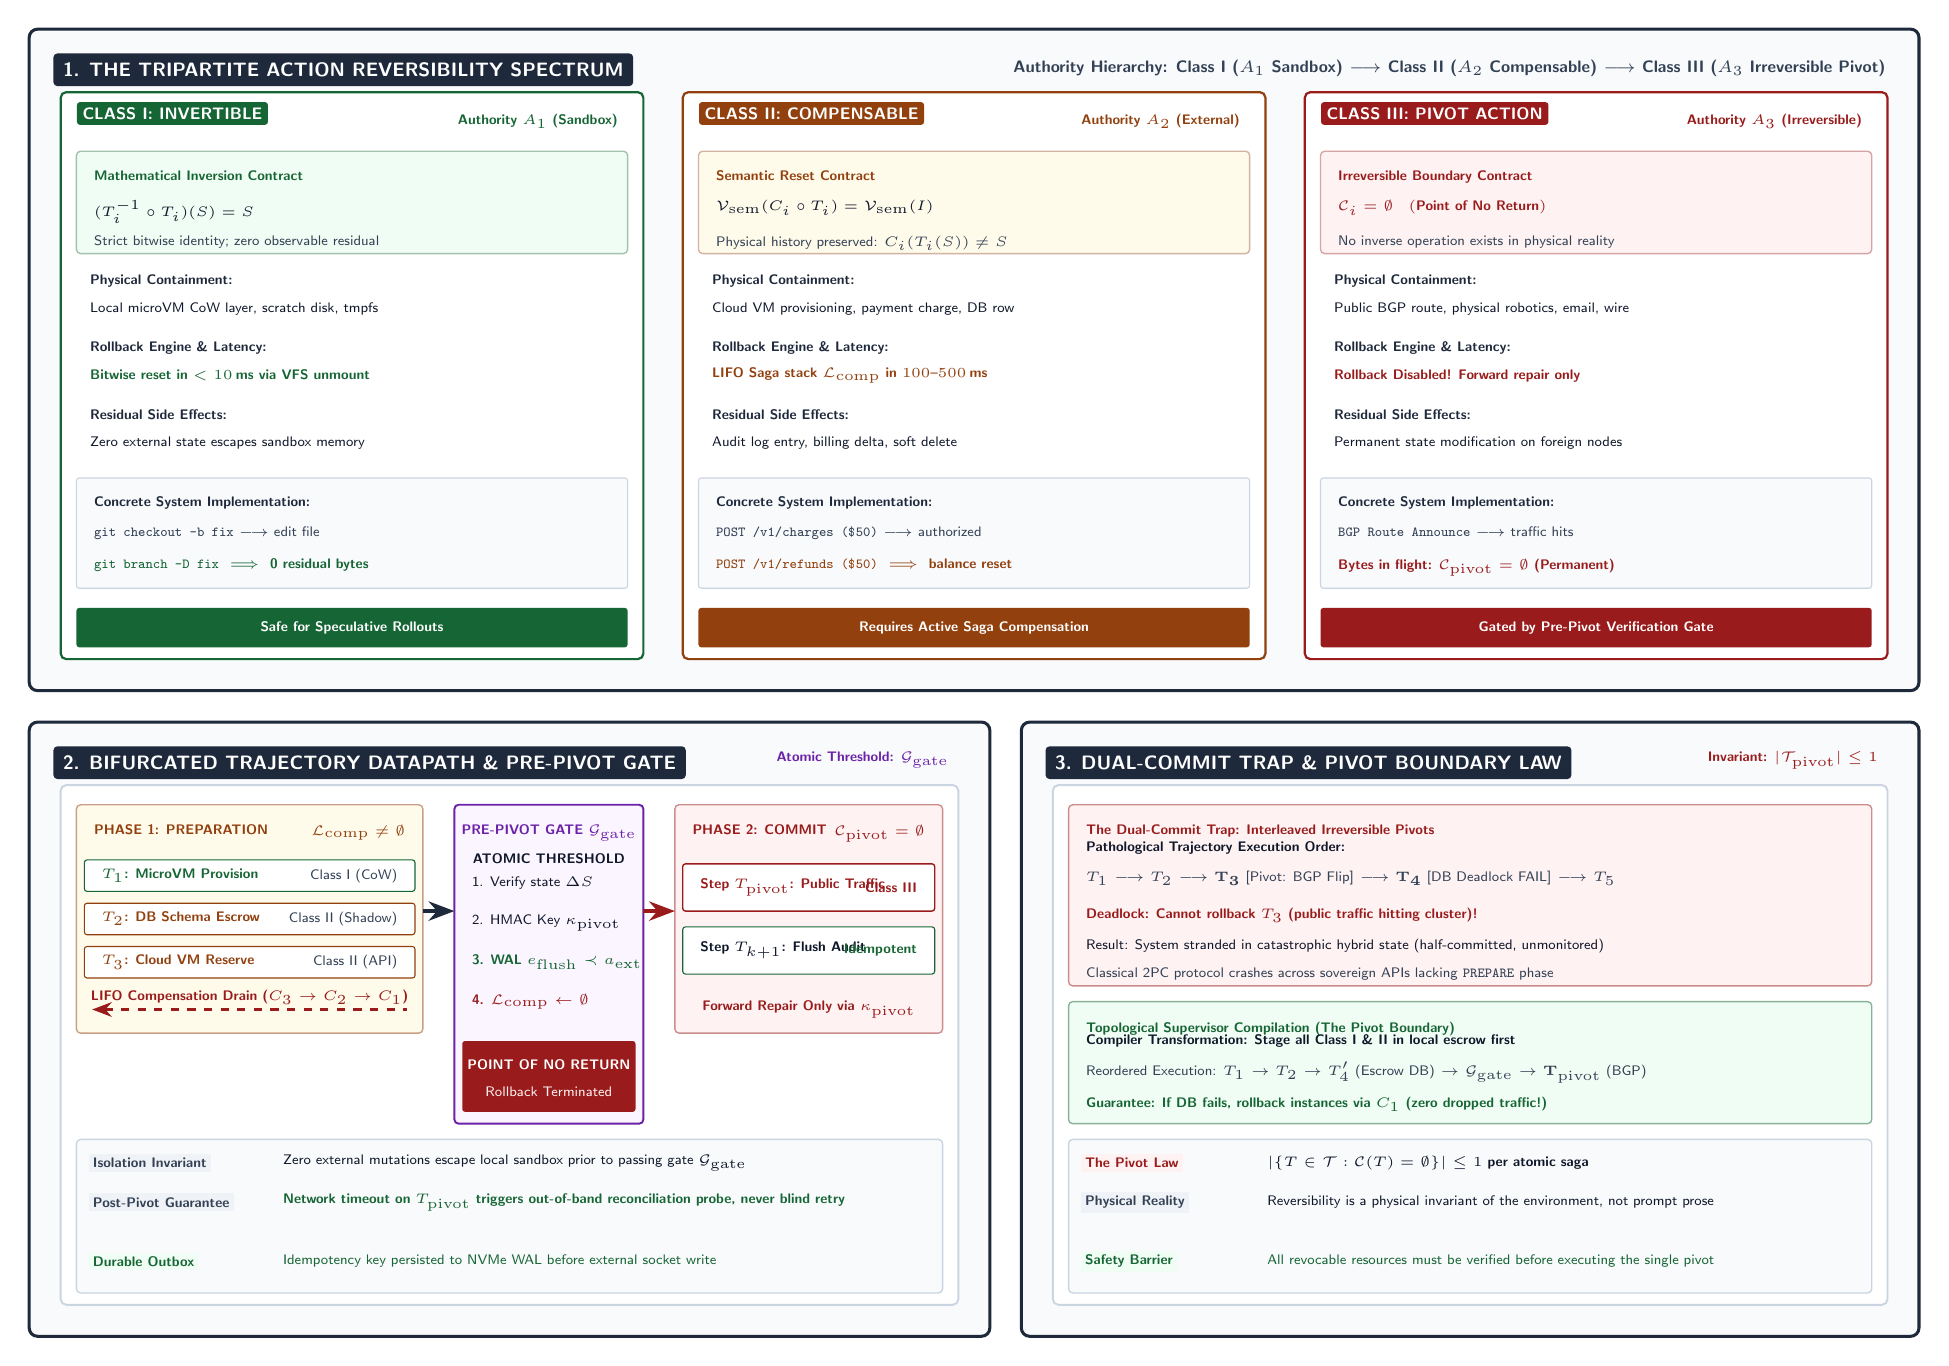
\begin{tikzpicture}[
  font=\sffamily,
  scale=1.0,
  >=Stealth,
  node distance=0.5cm
]

% =============================================================================
% TOP TIER: TRIPARTITE ACTION REVERSIBILITY TAXONOMY (y: 8.2 to 16.6)
% =============================================================================
\begin{scope}[shift={(0, 8.2)}]
  \draw[fill=CoolParchment, draw=OxfordNavy, line width=1.1pt, rounded corners=3pt]
    (0, 0) rectangle (24.0, 8.4);

  % Top Headers
  \node[anchor=north west, fill=OxfordNavy, text=white, font=\fontsize{7.5}{9.0}\selectfont\bfseries, rounded corners=1.5pt, inner sep=3.5pt]
    at (0.3, 8.1) {1. THE TRIPARTITE ACTION REVERSIBILITY SPECTRUM};
  \node[anchor=east, text=SlateSteel, font=\fontsize{6.0}{7.2}\selectfont\bfseries]
    at (23.7, 7.9) {Authority Hierarchy: Class I ($A_1$ Sandbox) $\longrightarrow$ Class II ($A_2$ Compensable) $\longrightarrow$ Class III ($A_3$ Irreversible Pivot)};

  % --- COLUMN 1: CLASS I - INVERTIBLE (x: 0.4 to 7.8) ---
  \begin{scope}[shift={(0.4, 0.4)}]
    \draw[fill=white, draw=ForestSage, line width=0.8pt, rounded corners=2pt] (0, 0) rectangle (7.4, 7.2);

    \node[anchor=north west, fill=ForestSage, text=white, font=\fontsize{5.8}{6.8}\selectfont\bfseries, rounded corners=1pt, inner sep=2pt]
      at (0.2, 7.08) {CLASS I: INVERTIBLE};
    \node[anchor=north east, font=\fontsize{4.6}{5.4}\selectfont\bfseries, text=ForestSage]
      at (7.2, 7.05) {Authority $A_1$ (Sandbox)};

    % Contract Box
    \draw[fill=SageL0, draw=ForestSage!40, line width=0.5pt, rounded corners=1.5pt] (0.2, 5.15) rectangle (7.2, 6.45);
    \node[anchor=north west, font=\fontsize{5.0}{6.0}\selectfont\bfseries, text=ForestSage] at (0.3, 6.32) {Mathematical Inversion Contract};
    \node[anchor=north west, font=\fontsize{4.9}{6.0}\selectfont\bfseries, text=DarkSlate] at (0.3, 5.95)
      {$(T_i^{-1} \circ T_i)(S) = S$};
    \node[anchor=north west, font=\fontsize{4.2}{5.0}\selectfont, text=SlateSteel] at (0.3, 5.50)
      {Strict bitwise identity; zero observable residual};

    % Specifications
    \node[anchor=west, font=\fontsize{4.5}{5.2}\selectfont\bfseries, text=OxfordNavy] at (0.25, 4.80) {Physical Containment:};
    \node[anchor=west, font=\fontsize{4.3}{5.1}\selectfont, text=DarkSlate] at (0.25, 4.45) {Local microVM CoW layer, scratch disk, tmpfs};

    \node[anchor=west, font=\fontsize{4.5}{5.2}\selectfont\bfseries, text=OxfordNavy] at (0.25, 3.95) {Rollback Engine \& Latency:};
    \node[anchor=west, font=\fontsize{4.3}{5.1}\selectfont\bfseries, text=ForestSage] at (0.25, 3.60) {Bitwise reset in $< 10\,\text{ms}$ via VFS unmount};

    \node[anchor=west, font=\fontsize{4.5}{5.2}\selectfont\bfseries, text=OxfordNavy] at (0.25, 3.10) {Residual Side Effects:};
    \node[anchor=west, font=\fontsize{4.3}{5.1}\selectfont, text=DarkSlate] at (0.25, 2.75) {Zero external state escapes sandbox memory};

    % Example Box
    \draw[fill=CoolParchment, draw=SlateRim, line width=0.4pt, rounded corners=1pt] (0.2, 0.90) rectangle (7.2, 2.30);
    \node[anchor=north west, font=\fontsize{4.5}{5.2}\selectfont\bfseries, text=OxfordNavy] at (0.3, 2.18) {Concrete System Implementation:};
    \node[anchor=north west, font=\fontsize{4.2}{5.0}\selectfont, text=SlateSteel] at (0.3, 1.80) {\texttt{git checkout -b fix} $\longrightarrow$ edit file};
    \node[anchor=north west, font=\fontsize{4.2}{5.0}\selectfont\bfseries, text=ForestSage] at (0.3, 1.40) {\texttt{git branch -D fix} $\implies$ 0 residual bytes};

    % Status Footer
    \draw[fill=ForestSage, draw=none, rounded corners=1pt] (0.2, 0.15) rectangle (7.2, 0.65);
    \node[anchor=center, font=\fontsize{4.4}{5.2}\selectfont\bfseries, text=white] at (3.7, 0.40) {Safe for Speculative Rollouts};
  \end{scope}

  % --- COLUMN 2: CLASS II - COMPENSABLE (x: 8.3 to 15.7) ---
  \begin{scope}[shift={(8.3, 0.4)}]
    \draw[fill=white, draw=WarmOchre, line width=0.8pt, rounded corners=2pt] (0, 0) rectangle (7.4, 7.2);

    \node[anchor=north west, fill=WarmOchre, text=white, font=\fontsize{5.8}{6.8}\selectfont\bfseries, rounded corners=1pt, inner sep=2pt]
      at (0.2, 7.08) {CLASS II: COMPENSABLE};
    \node[anchor=north east, font=\fontsize{4.6}{5.4}\selectfont\bfseries, text=WarmOchre]
      at (7.2, 7.05) {Authority $A_2$ (External)};

    % Contract Box
    \draw[fill=OchreL0, draw=WarmOchre!40, line width=0.5pt, rounded corners=1.5pt] (0.2, 5.15) rectangle (7.2, 6.45);
    \node[anchor=north west, font=\fontsize{5.0}{6.0}\selectfont\bfseries, text=WarmOchre] at (0.3, 6.32) {Semantic Reset Contract};
    \node[anchor=north west, font=\fontsize{4.9}{6.0}\selectfont\bfseries, text=DarkSlate] at (0.3, 5.95)
      {$\mathcal{V}_{\mathrm{sem}}(C_i \circ T_i) = \mathcal{V}_{\mathrm{sem}}(I)$};
    \node[anchor=north west, font=\fontsize{4.2}{5.0}\selectfont, text=SlateSteel] at (0.3, 5.50)
      {Physical history preserved: $C_i(T_i(S)) \ne S$};

    % Specifications
    \node[anchor=west, font=\fontsize{4.5}{5.2}\selectfont\bfseries, text=OxfordNavy] at (0.25, 4.80) {Physical Containment:};
    \node[anchor=west, font=\fontsize{4.3}{5.1}\selectfont, text=DarkSlate] at (0.25, 4.45) {Cloud VM provisioning, payment charge, DB row};

    \node[anchor=west, font=\fontsize{4.5}{5.2}\selectfont\bfseries, text=OxfordNavy] at (0.25, 3.95) {Rollback Engine \& Latency:};
    \node[anchor=west, font=\fontsize{4.3}{5.1}\selectfont\bfseries, text=WarmOchre] at (0.25, 3.60) {LIFO Saga stack $\mathcal{L}_{\mathrm{comp}}$ in $100\text{--}500\,\text{ms}$};

    \node[anchor=west, font=\fontsize{4.5}{5.2}\selectfont\bfseries, text=OxfordNavy] at (0.25, 3.10) {Residual Side Effects:};
    \node[anchor=west, font=\fontsize{4.3}{5.1}\selectfont, text=DarkSlate] at (0.25, 2.75) {Audit log entry, billing delta, soft delete};

    % Example Box
    \draw[fill=CoolParchment, draw=SlateRim, line width=0.4pt, rounded corners=1pt] (0.2, 0.90) rectangle (7.2, 2.30);
    \node[anchor=north west, font=\fontsize{4.5}{5.2}\selectfont\bfseries, text=OxfordNavy] at (0.3, 2.18) {Concrete System Implementation:};
    \node[anchor=north west, font=\fontsize{4.2}{5.0}\selectfont, text=SlateSteel] at (0.3, 1.80) {\texttt{POST /v1/charges (\$50)} $\longrightarrow$ authorized};
    \node[anchor=north west, font=\fontsize{4.2}{5.0}\selectfont\bfseries, text=WarmOchre] at (0.3, 1.40) {\texttt{POST /v1/refunds (\$50)} $\implies$ balance reset};

    % Status Footer
    \draw[fill=WarmOchre, draw=none, rounded corners=1pt] (0.2, 0.15) rectangle (7.2, 0.65);
    \node[anchor=center, font=\fontsize{4.4}{5.2}\selectfont\bfseries, text=white] at (3.7, 0.40) {Requires Active Saga Compensation};
  \end{scope}

  % --- COLUMN 3: CLASS III - PIVOT ACTION (x: 16.2 to 23.6) ---
  \begin{scope}[shift={(16.2, 0.4)}]
    \draw[fill=white, draw=Burgundy, line width=0.8pt, rounded corners=2pt] (0, 0) rectangle (7.4, 7.2);

    \node[anchor=north west, fill=Burgundy, text=white, font=\fontsize{5.8}{6.8}\selectfont\bfseries, rounded corners=1pt, inner sep=2pt]
      at (0.2, 7.08) {CLASS III: PIVOT ACTION};
    \node[anchor=north east, font=\fontsize{4.6}{5.4}\selectfont\bfseries, text=Burgundy]
      at (7.2, 7.05) {Authority $A_3$ (Irreversible)};

    % Contract Box
    \draw[fill=BurgundyL0, draw=Burgundy!40, line width=0.5pt, rounded corners=1.5pt] (0.2, 5.15) rectangle (7.2, 6.45);
    \node[anchor=north west, font=\fontsize{5.0}{6.0}\selectfont\bfseries, text=Burgundy] at (0.3, 6.32) {Irreversible Boundary Contract};
    \node[anchor=north west, font=\fontsize{4.9}{6.0}\selectfont\bfseries, text=Burgundy] at (0.3, 5.95)
      {$\mathcal{C}_i = \emptyset \quad (\text{Point of No Return})$};
    \node[anchor=north west, font=\fontsize{4.2}{5.0}\selectfont, text=SlateSteel] at (0.3, 5.50)
      {No inverse operation exists in physical reality};

    % Specifications
    \node[anchor=west, font=\fontsize{4.5}{5.2}\selectfont\bfseries, text=OxfordNavy] at (0.25, 4.80) {Physical Containment:};
    \node[anchor=west, font=\fontsize{4.3}{5.1}\selectfont, text=DarkSlate] at (0.25, 4.45) {Public BGP route, physical robotics, email, wire};

    \node[anchor=west, font=\fontsize{4.5}{5.2}\selectfont\bfseries, text=OxfordNavy] at (0.25, 3.95) {Rollback Engine \& Latency:};
    \node[anchor=west, font=\fontsize{4.3}{5.1}\selectfont\bfseries, text=Burgundy] at (0.25, 3.60) {Rollback Disabled! Forward repair only};

    \node[anchor=west, font=\fontsize{4.5}{5.2}\selectfont\bfseries, text=OxfordNavy] at (0.25, 3.10) {Residual Side Effects:};
    \node[anchor=west, font=\fontsize{4.3}{5.1}\selectfont, text=DarkSlate] at (0.25, 2.75) {Permanent state modification on foreign nodes};

    % Example Box
    \draw[fill=CoolParchment, draw=SlateRim, line width=0.4pt, rounded corners=1pt] (0.2, 0.90) rectangle (7.2, 2.30);
    \node[anchor=north west, font=\fontsize{4.5}{5.2}\selectfont\bfseries, text=OxfordNavy] at (0.3, 2.18) {Concrete System Implementation:};
    \node[anchor=north west, font=\fontsize{4.2}{5.0}\selectfont, text=SlateSteel] at (0.3, 1.80) {\texttt{BGP Route Announce} $\longrightarrow$ traffic hits};
    \node[anchor=north west, font=\fontsize{4.2}{5.0}\selectfont\bfseries, text=Burgundy] at (0.3, 1.40) {Bytes in flight: $\mathcal{C}_{\mathrm{pivot}} = \emptyset$ (Permanent)};

    % Status Footer
    \draw[fill=Burgundy, draw=none, rounded corners=1pt] (0.2, 0.15) rectangle (7.2, 0.65);
    \node[anchor=center, font=\fontsize{4.4}{5.2}\selectfont\bfseries, text=white] at (3.7, 0.40) {Gated by Pre-Pivot Verification Gate};
  \end{scope}

\end{scope}

% =============================================================================
% BOTTOM-LEFT (PANEL 2): BIFURCATED TRAJECTORY DATAPATH & PRE-PIVOT GATE
% =============================================================================
\begin{scope}[shift={(0, 0)}]
  \draw[fill=CoolParchment, draw=OxfordNavy, line width=1.1pt, rounded corners=3pt]
    (0, 0) rectangle (12.2, 7.8);

  % Inner White Box
  \begin{scope}[shift={(0.4, 0.4)}]
    \draw[fill=white, draw=SlateRim, line width=0.7pt, rounded corners=2pt] (0, 0) rectangle (11.4, 6.6);

    % Datapath Flow
    % Phase 1 Box (Preparation)
    \draw[fill=OchreL0, draw=WarmOchre!50, line width=0.5pt, rounded corners=1.5pt] (0.2, 3.45) rectangle (4.6, 6.35);
    \node[anchor=north west, font=\fontsize{4.8}{5.8}\selectfont\bfseries, text=WarmOchre] at (0.3, 6.22) {PHASE 1: PREPARATION};
    \node[anchor=north east, font=\fontsize{4.2}{5.0}\selectfont\bfseries, text=WarmOchre] at (4.5, 6.22) {$\mathcal{L}_{\mathrm{comp}} \ne \emptyset$};

    % Forward Steps
    \draw[fill=white, draw=ForestSage, line width=0.4pt, rounded corners=1pt] (0.3, 5.25) rectangle (4.5, 5.65);
    \node[anchor=west, font=\fontsize{4.2}{5.0}\selectfont\bfseries, text=ForestSage] at (0.4, 5.45) {$T_1$: MicroVM Provision};
    \node[anchor=east, font=\fontsize{4.0}{4.8}\selectfont, text=SlateSteel] at (4.4, 5.45) {Class I (CoW)};

    \draw[fill=white, draw=WarmOchre, line width=0.4pt, rounded corners=1pt] (0.3, 4.70) rectangle (4.5, 5.10);
    \node[anchor=west, font=\fontsize{4.2}{5.0}\selectfont\bfseries, text=WarmOchre] at (0.4, 4.90) {$T_2$: DB Schema Escrow};
    \node[anchor=east, font=\fontsize{4.0}{4.8}\selectfont, text=SlateSteel] at (4.4, 4.90) {Class II (Shadow)};

    \draw[fill=white, draw=WarmOchre, line width=0.4pt, rounded corners=1pt] (0.3, 4.15) rectangle (4.5, 4.55);
    \node[anchor=west, font=\fontsize{4.2}{5.0}\selectfont\bfseries, text=WarmOchre] at (0.4, 4.35) {$T_3$: Cloud VM Reserve};
    \node[anchor=east, font=\fontsize{4.0}{4.8}\selectfont, text=SlateSteel] at (4.4, 4.35) {Class II (API)};

    % Compensation unwind bar
    \draw[<-, draw=Burgundy, dashed, line width=0.9pt] (0.4, 3.75) -- (4.4, 3.75);
    \node[anchor=center, font=\fontsize{3.8}{4.5}\selectfont\bfseries, text=Burgundy] at (2.4, 3.90) {LIFO Compensation Drain ($C_3 \to C_2 \to C_1$)};

    % Pre-Pivot Gate Box
    \draw[fill=AmethystL0, draw=Amethyst, line width=0.7pt, rounded corners=1.5pt] (5.0, 2.30) rectangle (7.4, 6.35);
    \node[anchor=north, font=\fontsize{4.5}{5.5}\selectfont\bfseries, text=Amethyst] at (6.2, 6.22) {PRE-PIVOT GATE $\mathcal{G}_{\mathrm{gate}}$};
    \node[anchor=north, font=\fontsize{4.0}{4.8}\selectfont\bfseries, text=DarkSlate] at (6.2, 5.85) {ATOMIC THRESHOLD};

    \node[anchor=west, font=\fontsize{4.0}{4.8}\selectfont, text=DarkSlate] at (5.1, 5.35) {1. Verify state $\Delta S$};
    \node[anchor=west, font=\fontsize{4.0}{4.8}\selectfont, text=DarkSlate] at (5.1, 4.85) {2. HMAC Key $\kappa_{\mathrm{pivot}}$};
    \node[anchor=west, font=\fontsize{4.0}{4.8}\selectfont\bfseries, text=ForestSage] at (5.1, 4.35) {3. WAL $e_{\mathrm{flush}} \prec a_{\mathrm{ext}}$};
    \node[anchor=west, font=\fontsize{4.0}{4.8}\selectfont\bfseries, text=Burgundy] at (5.1, 3.85) {4. $\mathcal{L}_{\mathrm{comp}} \leftarrow \emptyset$};

    \draw[fill=Burgundy, draw=none, rounded corners=1pt] (5.1, 2.45) rectangle (7.3, 3.35);
    \node[anchor=center, font=\fontsize{3.8}{4.5}\selectfont\bfseries, text=white] at (6.2, 3.05) {POINT OF NO RETURN};
    \node[anchor=center, font=\fontsize{3.6}{4.2}\selectfont, text=BurgundyL0] at (6.2, 2.70) {Rollback Terminated};

    % Phase 2 Box (Commit / Execution)
    \draw[fill=BurgundyL0, draw=Burgundy!50, line width=0.5pt, rounded corners=1.5pt] (7.8, 3.45) rectangle (11.2, 6.35);
    \node[anchor=north west, font=\fontsize{4.6}{5.6}\selectfont\bfseries, text=Burgundy] at (7.9, 6.22) {PHASE 2: COMMIT};
    \node[anchor=north east, font=\fontsize{4.0}{4.8}\selectfont\bfseries, text=Burgundy] at (11.1, 6.22) {$\mathcal{C}_{\mathrm{pivot}} = \emptyset$};

    \draw[fill=white, draw=Burgundy, line width=0.5pt, rounded corners=1pt] (7.9, 5.00) rectangle (11.1, 5.60);
    \node[anchor=west, font=\fontsize{4.4}{5.2}\selectfont\bfseries, text=Burgundy] at (8.0, 5.30) {Step $T_{\mathrm{pivot}}$: Public Traffic};
    \node[anchor=east, font=\fontsize{4.0}{4.8}\selectfont\bfseries, text=Burgundy] at (11.0, 5.30) {Class III};

    \draw[fill=white, draw=ForestSage, line width=0.4pt, rounded corners=1pt] (7.9, 4.20) rectangle (11.1, 4.80);
    \node[anchor=west, font=\fontsize{4.4}{5.2}\selectfont\bfseries, text=DarkSlate] at (8.0, 4.50) {Step $T_{k+1}$: Flush Audit};
    \node[anchor=east, font=\fontsize{4.0}{4.8}\selectfont\bfseries, text=ForestSage] at (11.0, 4.50) {Idempotent};

    \node[anchor=center, font=\fontsize{3.8}{4.5}\selectfont\bfseries, text=Burgundy] at (9.5, 3.75) {Forward Repair Only via $\kappa_{\mathrm{pivot}}$};

    % Connectors
    \draw[->, line width=1.4pt, draw=OxfordNavy] (4.6, 5.0) -- (5.0, 5.0);
    \draw[->, line width=1.4pt, draw=Burgundy] (7.4, 5.0) -- (7.8, 5.0);

    % Structured Key-Value Specification Grid
    \begin{scope}[shift={(0.2, 0.15)}]
      \draw[fill=CoolParchment, draw=SlateRim, line width=0.5pt, rounded corners=1.5pt] (0, 0) rectangle (11.0, 1.95);

      \node[anchor=west, fill=SlateRim!30, text=SlateSteel, font=\fontsize{4.5}{5.2}\selectfont\bfseries, inner sep=1.5pt] at (0.15, 1.65) {Isolation Invariant};
      \node[anchor=west, font=\fontsize{4.5}{5.3}\selectfont, text=DarkSlate] at (2.5, 1.65) {Zero external mutations escape local sandbox prior to passing gate $\mathcal{G}_{\mathrm{gate}}$};

      \node[anchor=west, fill=SlateRim!30, text=SlateSteel, font=\fontsize{4.5}{5.2}\selectfont\bfseries, inner sep=1.5pt] at (0.15, 1.15) {Post-Pivot Guarantee};
      \node[anchor=west, font=\fontsize{4.5}{5.3}\selectfont\bfseries, text=ForestSage] at (2.5, 1.15) {Network timeout on $T_{\mathrm{pivot}}$ triggers out-of-band reconciliation probe, never blind retry};

      \node[anchor=west, fill=SageL0, text=ForestSage, font=\fontsize{4.5}{5.2}\selectfont\bfseries, inner sep=1.5pt] at (0.15, 0.40) {Durable Outbox};
      \node[anchor=west, font=\fontsize{4.5}{5.3}\selectfont, text=ForestSage] at (2.5, 0.40) {Idempotency key persisted to NVMe WAL before external socket write};
    \end{scope}

  \end{scope}

  % Header Badges Drawn on Top of Base
  \node[anchor=north west, fill=OxfordNavy, text=white, font=\fontsize{7.5}{9.0}\selectfont\bfseries, rounded corners=1.5pt, inner sep=3.5pt]
    at (0.3, 7.5) {2. BIFURCATED TRAJECTORY DATAPATH \& PRE-PIVOT GATE};
  \node[anchor=east, text=Amethyst, font=\fontsize{5.5}{6.8}\selectfont\bfseries]
    at (11.8, 7.32) {Atomic Threshold: $\mathcal{G}_{\mathrm{gate}}$};

\end{scope}

% =============================================================================
% BOTTOM-RIGHT (PANEL 3): DUAL-COMMIT TRAP & PIVOT BOUNDARY LAW
% =============================================================================
\begin{scope}[shift={(12.6, 0)}]
  \draw[fill=CoolParchment, draw=OxfordNavy, line width=1.1pt, rounded corners=3pt]
    (0, 0) rectangle (11.4, 7.8);

  % Inner White Box
  \begin{scope}[shift={(0.4, 0.4)}]
    \draw[fill=white, draw=SlateRim, line width=0.7pt, rounded corners=2pt] (0, 0) rectangle (10.6, 6.6);

    % The Dual-Commit Trap Box
    \draw[fill=BurgundyL0, draw=Burgundy!50, line width=0.5pt, rounded corners=1.5pt] (0.2, 4.05) rectangle (10.4, 6.35);
    \node[anchor=north west, font=\fontsize{5.0}{6.0}\selectfont\bfseries, text=Burgundy] at (0.3, 6.22) {The Dual-Commit Trap: Interleaved Irreversible Pivots};

    \node[anchor=west, font=\fontsize{4.4}{5.2}\selectfont\bfseries, text=DarkSlate] at (0.3, 5.80) {Pathological Trajectory Execution Order:};
    \node[anchor=west, font=\fontsize{4.2}{5.0}\selectfont, text=SlateSteel] at (0.3, 5.42)
      {$T_1 \longrightarrow T_2 \longrightarrow \mathbf{T_3\text{ [Pivot: BGP Flip]}} \longrightarrow \mathbf{T_4\text{ [DB Deadlock FAIL]}} \longrightarrow T_5$};

    \node[anchor=west, font=\fontsize{4.3}{5.1}\selectfont\bfseries, text=Burgundy] at (0.3, 4.95)
      {Deadlock: Cannot rollback $T_3$ (public traffic hitting cluster)!};
    \node[anchor=west, font=\fontsize{4.2}{5.0}\selectfont, text=DarkSlate] at (0.3, 4.55)
      {Result: System stranded in catastrophic hybrid state (half-committed, unmonitored)};
    \node[anchor=west, font=\fontsize{4.1}{4.9}\selectfont, text=SlateSteel] at (0.3, 4.20)
      {Classical 2PC protocol crashes across sovereign APIs lacking \texttt{PREPARE} phase};

    % Topological Supervisor Compilation Box
    \draw[fill=SageL0, draw=ForestSage!50, line width=0.5pt, rounded corners=1.5pt] (0.2, 2.30) rectangle (10.4, 3.85);
    \node[anchor=north west, font=\fontsize{5.0}{6.0}\selectfont\bfseries, text=ForestSage] at (0.3, 3.72) {Topological Supervisor Compilation (The Pivot Boundary)};

    \node[anchor=west, font=\fontsize{4.4}{5.2}\selectfont\bfseries, text=DarkSlate] at (0.3, 3.35)
      {Compiler Transformation: Stage all Class I \& II in local escrow first};
    \node[anchor=west, font=\fontsize{4.3}{5.1}\selectfont, text=SlateSteel] at (0.3, 2.95)
      {Reordered Execution: $T_1 \to T_2 \to T_4' \text{ (Escrow DB)} \to \mathcal{G}_{\mathrm{gate}} \to \mathbf{T_{\mathrm{pivot}}\text{ (BGP)}}$};
    \node[anchor=west, font=\fontsize{4.3}{5.1}\selectfont\bfseries, text=ForestSage] at (0.3, 2.55)
      {Guarantee: If DB fails, rollback instances via $C_1$ (zero dropped traffic!)};

    % Structured Key-Value Specification Grid
    \begin{scope}[shift={(0.2, 0.15)}]
      \draw[fill=CoolParchment, draw=SlateRim, line width=0.5pt, rounded corners=1.5pt] (0, 0) rectangle (10.2, 1.95);

      \node[anchor=west, fill=BurgundyL0, text=Burgundy, font=\fontsize{4.5}{5.2}\selectfont\bfseries, inner sep=1.5pt] at (0.15, 1.65) {The Pivot Law};
      \node[anchor=west, font=\fontsize{4.5}{5.3}\selectfont\bfseries, text=DarkSlate] at (2.4, 1.65)
        {$|\{T \in \mathcal{T} : \mathcal{C}(T) = \emptyset\}| \le 1$ per atomic saga};

      \node[anchor=west, fill=SlateRim!30, text=SlateSteel, font=\fontsize{4.5}{5.2}\selectfont\bfseries, inner sep=1.5pt] at (0.15, 1.15) {Physical Reality};
      \node[anchor=west, font=\fontsize{4.5}{5.3}\selectfont, text=DarkSlate] at (2.4, 1.15) {Reversibility is a physical invariant of the environment, not prompt prose};

      \node[anchor=west, fill=SageL0, text=ForestSage, font=\fontsize{4.5}{5.2}\selectfont\bfseries, inner sep=1.5pt] at (0.15, 0.40) {Safety Barrier};
      \node[anchor=west, font=\fontsize{4.5}{5.3}\selectfont, text=ForestSage] at (2.4, 0.40) {All revocable resources must be verified before executing the single pivot};
    \end{scope}

  \end{scope}

  % Header Badges Drawn on Top of Base
  \node[anchor=north west, fill=OxfordNavy, text=white, font=\fontsize{7.5}{9.0}\selectfont\bfseries, rounded corners=1.5pt, inner sep=3.5pt]
    at (0.3, 7.5) {3. DUAL-COMMIT TRAP \& PIVOT BOUNDARY LAW};
  \node[anchor=east, text=Burgundy, font=\fontsize{5.5}{6.8}\selectfont\bfseries]
    at (11.0, 7.32) {Invariant: $|\mathcal{T}_{\mathrm{pivot}}| \le 1$};

\end{scope}

\end{tikzpicture}
\end{document}
